\section{Обзор предметной области}
\label{sec:domain:intro}

В данном разделе будет произведён обзор предметной области задачи, решаемой в рамках дипломного проекта - аутентификации цифровых устройств как механизма обеспечения информационной безопасности и контроля доступа к конфиденциальным данным и ресурсам; рассмотрены существующие методы аутентификации цифровых устройств с использованием физически неклонируемых функций, как теоретические, так и применяемые на практике; приведены преимущества и недостатки различных подходов, используемых при проектировании цифровых устройств и систем их аутентификации.
В частности, будут рассмотрены варианты использования уникальных неклонируемых идентификаторов в протоколах аутентификации цифровых устройств.

\subsection{Физически неклонируемые функции}
\label{sub:domain:pufs}
Физическая криптография, в основе которой лежат физически неклонируемые функции, находит применение не только в традиционном смысле защиты конфиденциальной информации, но также и в области защиты собственно электронных цифровых устройств от несанкционированного использования, изменения, клонирования.

Идея использования физически неклонируемых функций (\emph{Phisycal Unclonable Function, PUF}, или изначально \emph{Physical One"=Way Function, POWF}) впервые была предложена в работах Р. Паппу (R. Pappu) в 2001 году~\cite{rpappu_powf}, а современное толкование и определение сформулировал П. Туилс (P. Tuyls) в 2006 году~\cite{ptuyls_pufs}. Согласно этому определению, физически неклонируемой функцией называют набор характеристик физической (цифровой) системы, копирование и воспроизведение которого применительно к другим физическим системам невозможно. Цифровые системы, как правило, состоят из множества компонент, физические параметры которых формируются на стадии производства и принимают случайные в некотором диапазоне значения. Контролировать эти значения невозможно в силу хаотичности микро- (а часто и макро-) скопических параметров физической системы, в рамках которой происходит создание устройства. Подобное свойство получило название физической вариации технологического процесса~\cite{ivaniuk_pufs}. Таким образом, уникальность и невоспроизводимость (неклонируемость) цифровой системы обеспечивается наличием подобных случайных параметров. Более того, PUF могут быть реализованы таким образом, который не допускает симуляцию, моделирование или предсказание их поведения. Идея использования PUF в криптографических целях основана на извлечении и использовании этих случайных параметров.

Физически неклонируемые функции - инновационные примитивы цифровых устройств, используемые в физической криптографии, которые, благодаря своим свойствам, имеют уникальные для каждого экземпляра функции. ФНФ во многом можно считать аналогами биометрических систем: в то время как последние основаны на уникальных биологических/физиологических свойствах каждого отдельного человека, ФНФ опирается на уникальные <<синтетические>> признаки интегрированных микросхем.

Благодаря способности превосходно генерировать и хранить секретную информацию, ФНФ могут служить отличным физическим каркасом для построения системы информационной безопасности. Неклонируемость и специфичность структуры каждого экземпляра позволяют использовать их в качестве уникальных идентификаторов различных сущностей. В совокупности с подходящими алгоритмами обработки информации их можно успешно использовать в системах аутентификации, в частности для генерации и хранения секретных последовательностей.


\def\crp {\left\{C_i, R_i\right\}}

PUF - это физическая система, которая при воздействии на неё (запросе) порождает уникальный, но непредсказуемый ответ. Специфический запрос C (\emph{Challenge}) и соответствующий ему выходной сигнал R (\emph{Response}) вместе образуют пару запрос"=ответ (\emph{Challenge"={}Response Pair, CRP}). PUF, в свою очередь, является функцией преобразования множества запросов $ C_i $ в множество ответов $ R_i $:
\begin{equation}
  \label{eq:domain:pufs:puf_main}
  R_i = PUF(C_i)
\end{equation}

По определению У. Рурмаира (U. Ruhrmair), PUF представляют собой сложные неуправляемые физические системы со сверхбольшим объёмом структурной информации (Super High Information Content, SHIC). PUF должны удовлетворять следующим свойствам:
\begin{enumerate}
  \item Физическое копирование системы с сохранением её свойств в виде пар $ \crp $ должно быть практически невозможно.
  \item Информация в виде ответов $ R_i $ на различные запросы $ C_i $ может быть извлечена из системы многократно и с высокой степенью надёжности.
  \item Множество возможных запросов $ C_i $ должно быть достаточно велико, чтобы получение всех возможных пар $ \crp $ не представлялось возможным за разумное время и количество ресурсов.
  \item Пары $ \crp $ должны быть независимы друг от друга в том смысле, что по известной паре $ \crp $ невозможно получить, смоделировать или предсказать значение любой другой пары или множества пар.
\end{enumerate}

Перечисленные свойства PUF обусловлены понятием \emph{вариации технологического процесса (Process Variation)}. Применительно к производству полупроводников, оно описывает естественные отклонения физических параметров транзисторов (длина, ширина, толщина оксидной плёнки) от заданных значений на этапе их изготовления. Вариация становится наиболее актуальное при производстве на уровне техпроцесса 65нм и менее, ведь с уплотнением техпроцесса подобные отклонения в процентном соотношении имеют всё большее влияние на конечные параметры элемента, размеры которого всё больше обусловлены размером атомов и длиной волны излучения, используемого, для формирования литографического трафарета.

Вариации технологического процесса подвержены любые полупроводниковые устройства, но в большей степени -- аналоговые микросхемы. И хотя вариация не является контролируемым процессом, она вполне может быть отслежена и сопоставлена с отклонениями в рабочих параметрах устройств в целях контроля качества, а в последствии, возможно, и скорректирована.


% Виды ФНФ

\subsection{Виды PUF по физической реализации. }
\label{sub:domain:puf_physical_types}


\subsubsection{PUF на оптических элементах. }
\label{sub:domain:puf_physical_types:optical}

Любые физически неклонируемые функции, в которых процесс реакции системы в основе своей имеет какое"=либо оптическое явление, называются оптическими.
Как правило, используется объект с неоднородной прозрачностью (подобно светоотражающим пузырькам из примера выше). Именно благодаря рассеивающему действию вещества и вкраплений объект не может быть исследован и смоделирован математически. Оптическое сканирование не может проникнуть вглубь объекта.
\begin{figure}[ht]
    \centering
    \label{fig:domain:puf_physical_types:optical}
    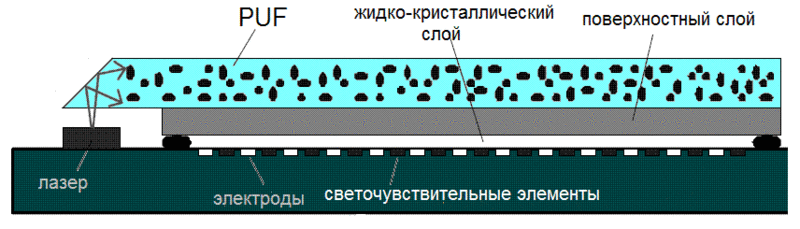
\includegraphics[width=0.7\textwidth]{optical.png}
    \caption{общая структура PUF на оптических элементах}
\end{figure}


\subsubsection{PUF на интегральных микросхемах. }
\label{sub:domain:puf_physical_types:ic}

Аналогично пузырькам в оптической системе, в иных средах тоже можно получить неклонируемость. Рассмотрим среду, и так широко используемую в цифровых устройствах - электрические проводники и диэлектрики.
Любое современное технологичное устройство содержит в себе внушительное количество интегральных микросхем. На них и построены PUF данного типа. Несмотря на то, что микросхемы изготавливаются по одному и тому же технологическому процессу, каждая из них достаточно уникальна для корректной работы PUF. Это может быть использовано в системах информационной безопасности как уникальный идентификационный признак устройства.
Один из вариантов построения такой PUF: интегральная микросхема покрывается слоем защитного вещества со вкраплениями диэлектрика. Эти вкрапления имеют случайные размер и форму. Под этот слой подводятся электроды"=датчики. В совокупности с защитным слоем каждый такой электрод обретает свойства конденсатора случайной (зависящей от вкраплений диэлектрика в защитный слой) ёмкости. Очевидно, что случайность ёмкости каждого конденсатора достигается при размере частиц, сравнимом с размером между электродами.


\subsubsection{PUF на полевых транзисторах. }
\label{sub:domain:puf_physical_types:transistors}

В основе таких PUF лежит особенность полевых транзисторов задерживать сигнал, проходящий по нему на непредсказуемое время, зависящее от физических свойств материала транзистора (именно из"=за материала такие PUF ещё называют кремниевыми). Физическая система PUF будет состоять из набора пар транзисторов и триггеров"=арбитров. Триггер будет давать на выход 0 или 1 в зависимости от того, сигнал с какого из пары транзисторов пришёл к нему раньше. Подавая на вход этому набору некоторый сигнал"=запрос, на выходе исследователь получит набор значений триггеров - реакцию системы на запрос, уникальную для данного устройства, в состав которого включаются упомянутые транзисторы. Неклонируемость строится на физической неидеальности процесса производства. Изучение функции для последующего математического прогноза реакции на запрос возможно только полным перебором входных сигналов, что является достаточно вычислительно сложной задачей.


\subsubsection{PUF на магнитных элементах. }
\label{sub:domain:puf_physical_types:magnetic}

Практическое применение - уникальный идентификатор магнитной полосы банковской карты. Частицы феррита бария, содержащиеся в пасте"=основе магнитной полосы, также имеют случайный размер и форму. Логично сделать вывод, что на случайности их распределения можно построить PUF. Неклонируемость снова опирается на физическую неидеальность процесса производства. Неточности и погрешности не дадут повторить рисунок частиц феррита бария в  точности. А математическое моделирование не препятствует выполнению данной PUF её задачи.
\begin{figure}[ht]
    \centering
    \label{fig:domain:puf_physical_types:magnetic}
    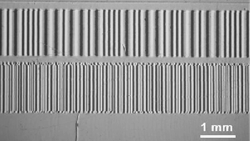
\includegraphics[width=0.55\textwidth]{magneticstripe.png}
    \caption{структура магнитной полосы -- варианта магнитной PUF}
\end{figure}

\subsection{Виды PUF по принципу работы. }
\label{sub:domain:puf_types}


\subsubsection{PUF типа арбитр (Arbiter PUF). }
\label{sub:domain:puf_types:arbiter}

Физически неклонируемые функции по типу арбитра - разновидность физически неклонируемых функций на основе задержек. Идея состоит в том, чтобы привнести состояние гонки между двумя путями микросхемы. Оба пути заканчиваются элементом"=арбитром, который определяет какой из путей был быстрее и выдает соответствующее бинарное значение.
\begin{figure}[ht]
    \centering
    \label{fig:domain:puf_types:arbiter}
    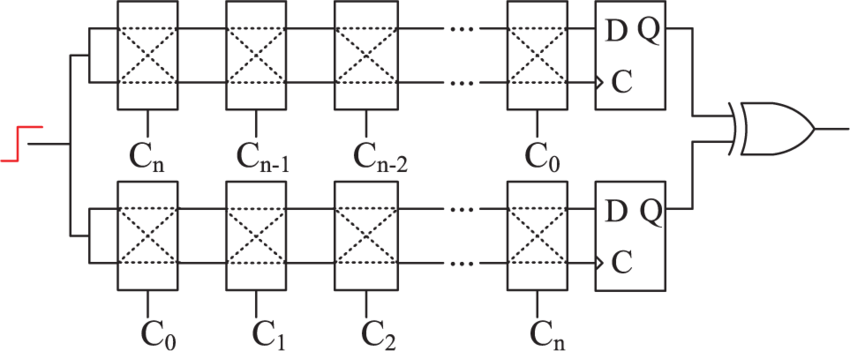
\includegraphics[width=0.7\textwidth]{arbiter.png}
    \caption{PUF типа арбитр}
\end{figure}

\subsubsection{PUF на базе кольцевого генератора (RO"=PUF). }
\label{sub:domain:puf_types:ring_oscillator}

Физически неклонируемые функции на базе кольцевых генераторов также используют неконтролируемые изменения задержек процессов цифровых компонентов в качестве источника случайности. Когда эти компоненты образуют кольцевой генератор, частоты его выходных сигналов различаются, что и используется при формировании бинарного ответа.
\begin{figure}[ht]
    \centering
    \label{fig:domain:puf_types:ring_oscillator}
    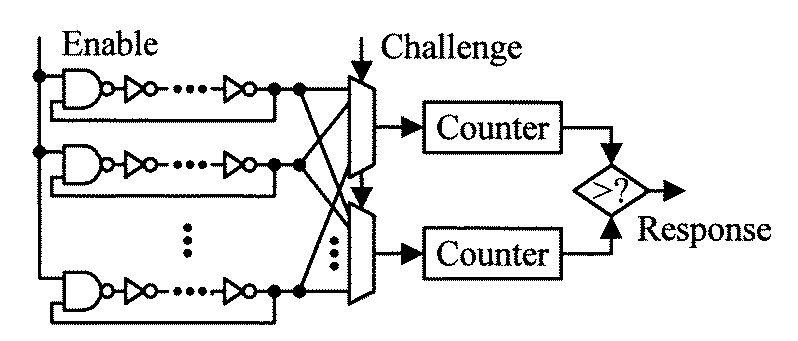
\includegraphics[width=0.7\textwidth]{ro-puf.png}
    \caption{PUF на базе кольцевого генератора}
\end{figure}


\subsubsection{PUF на основе сбоев (Failure PUF). }
\label{sub:domain:puf_types:failure_puf}

Этот тип физически неклонируемых функций основываются на сбоях в поведении комбинаторных логических схем. В идеале у комбинаторной схемы нет внутреннего состояния, что означает, что стационарный выход полностью определяется его входными сигналами. Однако, когда логическое значение на входе изменяется, для достижения стационарного значения на выходе требуется некоторое время. Появление сбоя определяется различиями в задержках различных логических цепей от входов к выходному сигналу. Так как задержки определенных образцов комбинаторных схем вызваны случайными изменениями процесса, появление, количество и форма сбоев выходных сигналов также будут случайными и характерными для определенных образцов схемы. Поэтому оценка поведения сбоев таких схем может быть использована для ответа физически неклонируемой функции.


\subsubsection{PUF типа <<бабочка>> (Butterfly PUF). }
\label{sub:domain:puf_types:butterfly}
Физически неклонируемые функции по типу бабочки имитирует работу ячейки СОЗУ, формируя перекрестные обратные связи для получения бистабильной схемы. Схема принудительно переводится в неустойчивое состояние, после чего схема переходит в одно из двух стабильных состояний, которое зависит от случайной разности задержек в паре линий обратной связи и линии входного сигнала.
\begin{figure}[ht]
    \centering
    \label{fig:domain:puf_types:butterfly}
    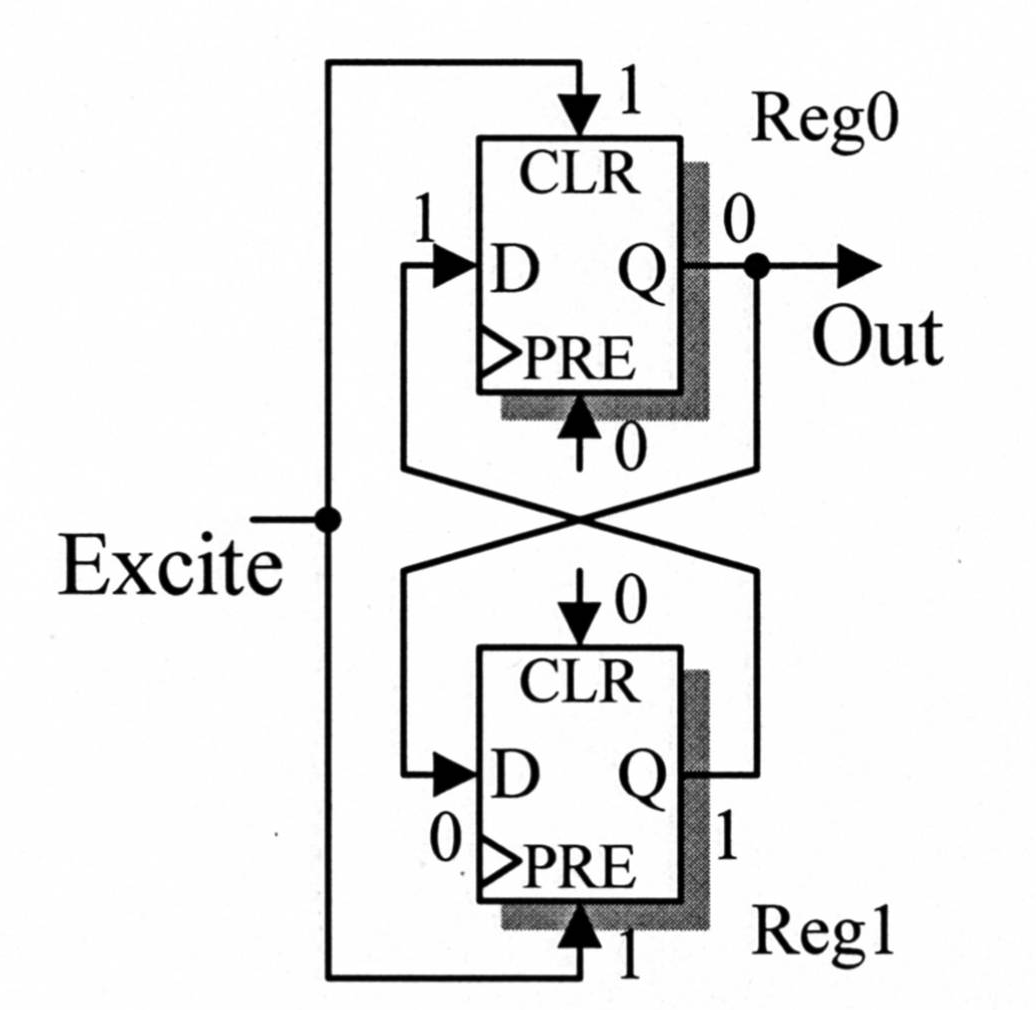
\includegraphics[width=0.5\textwidth]{butterfly.png}
    \caption{PUF типа <<бабочка>>}
\end{figure}


\subsubsection{PUF на базе SRAM (SRAM PUF). }
\label{sub:domain:puf_types:sram}
Принцип работы физически неклонируемых функций на базе статического оперативного запоминающего устройства (СОЗУ) основан на случайности состояния части ячеек СОЗУ при включении.

Стоит заметить, что в данном списке перечислены лишь базовые варианты реализации PUF. На их основе и на основе комбинаций этих типов может быть построено огромное множество различных сложных PUF. ~\cite{cryptowiki_pufs, rmaes_pufs}


\subsection{Использование PUF для идентификации и аутентификации цифровых устройств}
\label{sub:domain:puf_auth}
Аутентификация традиционно характеризуется как процесс проверки того, что сущность владеет конкретной информацией, например, паролем, обладает конкретными свойствами, или же является именно тем, за что (кого) себя выдает. Многофакторная аутентификация
представляет собой комбинацию этих проверок. Аутентификация на основе физически неклонируемых функций подразумевает наличие разных независимых устройств, каждое из которых характеризуется набором паролей (т.е. в данном случае -- набором пар запрос"=ответ), который однозначно идентифицирует эти устройства, то есть, в какой-то степени, аутентификацию на основе PUF можно считать многофакторным механизмом.

Множество возможных применений ФНФ также включает шифрование информации, обнаружение вредоносных изменений структуры интегральной микросхемы, контроль специфических функций устройств и многие другие. Каждый из сценариев использования предъявляет определенные требования к свойствам используемой ФНФ. В частности, для использования в криптографических целях, ФНФ должна быть устойчива к атакам моделирования, т.е. должна препятствовать построению более-менее точной модели своей структуры и/или поведения. Это же применимо и к протоколам аутентификации на основе ФНФ. Общее правило -- чем больше контроля над своими входными и выходными параметрами ФНФ предоставляет программному или аппаратному приложению, тем лучше оно должно быть защищено от таких атак.

Применительно к аутентификации на основе ФНФ применяют термины \emph{электронный ключ (токен)} -- для обозначения утройства, оснащённого ФНФ, чья подлинность проверяется, например, смарт-карта или RFID-метка, и \emph{доверенный сервер} -- для обозначения стороны, располагающей истинными данными идентификации конкретных устройств.

Существует два основных подхода к осуществлению системы аутентификации, основанной на физически неклонируемых функциях. Первый подход состоит в получении стойкого и безопасного криптографического ключа из ответа физически неклонируемой функции и использовании этого ключа в каком"=либо из существующих криптографических протоколов аутентификации. В этом случае ФНФ используется в качестве или как составная часть генератора истинно случайных чисел с показателями, достаточными для его применения в криптографических целях. Секретность ключа повышается тем, что в открытом виде могут храниться только данные, использованые для его генерации, в данном случае -- наборы пар $\crp$. Следовательно, воспроизвести ключ возможно только при использовании исходной ФНФ и с данным набором входных данных. Для этого подхода достаточно довольно простой ФНФ (т.н. \emph{weak PUF, слабая ФНФ}), способной сгенерировать небольшое количество случайной информации, но при этом устройство должно содержать реализацию криптографического алгоритма, чтобы из входного набора сконструировать ключ. К сожалению, этот метод уязвим к атаке по стороннему каналу (side-channel attack): злоумышленник может получить секретный ключ, используя уязвимости в аппаратной реализации алгоритма.

Другой подход состоит в разработке схемы аутентификации, которая напрямую применяет уникальность и непредсказуемость поведения пары запроса"=ответа отдельного объекта. Такая схема состоит из двух фаз (регистрации и подтверждения):

В первой фазе, каждый объект проходит регистрацию у проверяющего. Во время этой фазы проверяющий записывает идентификатор каждого объекта и собирает значительное подмножество пар запрос"=ответ каждого объекта (устройства) для случайно сгенерированных запросов. Собранные пары запрос"=ответ хранятся в базе данных проверяющего.

Во время фазы подтверждения, объект (устройство) посылает проверяющему свой идентификатор. Проверяющий находит его в базе данных, выбирает оттуда случайную пару запрос"=ответ, которая соответствует полученному идентификатору. Запрос посылается объекту, объект вычисляет физически неклонируемую функцию и посылает ответ. Проверяющий сравнивает этот ответ со значением из базы данных, и если проверка прошла успешно, тообъект аутентифицирован, иначе -- аутентификация отклонена. Использованная пара запрос"=ответ удаляется из базы данных для исключения возможности сохранения результатов третьей стороной. Корректность данной схемы аутентификации обеспечивается тем фактом, что ответы физически неклонируемых функций воспроизводимы самим объектом в течение долгого времени.
Однако, этот подход в описанном выше виде имеет существенные недостатки:
\begin{itemize}
  \item Число возможных пар $ \crp $ может быть очень большим. Вследствие этого, регистрация устройства путем сбора достаточного для последуещей аутентификации количества пар не всегда возможно за приемлемое время.
  \item Несмотря на то, что ответы физически неклонируемых функций воспроизводимы самим объектом, ФНФ редко являются полностью стабильными. Подавляющее большинство реализаций имеют дополнительную зависимость выходного сигнала от побочных эффектов, таких как физический износ устройства, температура окружающей среды, влажность и других параметров. В связи с этим, однозначное соответствие нескольких выходных сигналов $ R $, вызванных одним набором $ C $, не может быть гарантировано.
\end{itemize}
Из-за этих нюансов, использование <<наивной>> реализации протокола не представляет особой практической ценности. Поэтому данный дипломный проект ставит целью исследование и реализацию усовершенствованного протокола аутентификации, учитывающего указанные особенности и предоставлящего достаточный уровень секретности и защиты от перехвата управления третьей стороной.


\subsection{Обзор существующих аналогов}
Подавляющее большинство средств защиты интеллектуальной собственности применительно к цифровым устройствам, в частности, программные средства аутентификации устройств на основе физически неклонируемых функций, а также особенности их реализации сами по себе являются коммерческой тайной. В связи с этим, даже поверхностный анализ и сравнение существующих аналогов не представляется возможным. Однако, целесообразным представляется создание доступного открытого аналога средства аутентификации, которое, в противовес проприетарным решениям компаний"=производителей, могло бы служить удобной базой для дальнейшей развития и затачивания под конкретные нужды энтузиастами разработки цифровых устройств, а также в образовательных целях.


\subsection{Постановка задачи}
В результате выполнения дипломного проекта должно быть разработано программное средство аутентификации цифровых устройств, реализующее протокол взаимодействия между сервером аутентификации и цифровым устройством, включающим в себя некоторую реализацию PUF для однозначной его идентификации.
\begin{itemize}
\item разрабатываемое ПО должно работать на операционных системах Linux и Windows;
\item программное средство должно быть выполнено в виде клиент"=серверного приложения;
\item программное средство должно поддерживать работу как в режиме регистрации устройства в базе данных, так и в режиме его аутентификации;
\item принцип работы разрабатываемого ПО не должен быть привязан к конкретному типу аутентифицируемого устройства.
\end{itemize}
